\part{INTRODUÇÃO}

\chapter[Introdução]{Introdução}



\section[Contexto]{Contexto}

Nos últimos anos temos visto iniciativas isoladas de algumas entidades da Administração Pública em procurar adotar métodos ágeis, com destaque para o Scrum e o Extreme Programming-XP, em suas equipes de desenvolvimento. Ainda mais recente, houve a iniciativa de mesclar o uso de métodos ágeis com a filosofia de gestão da produção, conhecida com LEAN, com o foco em gerenciar o contrato dos fornecedores de desenvolvimento de software.

Lean no Desenvolvimento de Software é uma filosofia que busca aplicar os princípios do Pensamento Lean no desenvolvimento do software. Dentre os princípios do Lean se destacam: a eliminação de desperdícios; o respeito às pessoas envolvidas no processo; a qualidade; a simplicidade; a otimização do todo e entregas rápidas. É importante ressaltar que apesar de sugerir diversas ferramentas, como o Kanban, também presente em Métodos Ágeis, o Lean está mais relacionado à forma de pensar, exige muito mais uma mudança cultural de cada organização do que a aplicação e utilização de ferramentas. 

Lean está relacionado com Métodos Ágeis, não só pela semelhança dos seus princípios e práticas, mas também porque ambos valorizam as pessoas em detrimento de ferramentas e buscam agregar valor de negócio ao sistema que está sendo desenvolvido. Do ponto de vista teórico os métodos ágeis e o Lean, se baseiam em diferentes teorias, como: teoria geral dos sistemas, teoria da complexidade e teoria das restrições. Essas teorias representam um contraponto a metodologias mais prescritivas e preditivas, também conhecidas como tradicionais, que possuem seu amparo teórico principalmente na visão da teoria da administração científica.

Scrum é uma metodologia ágil desenvolvida para a gestão do processo de desenvolvimento de software. É uma abordagem que aplica ideias de controle de processos da indústria ao desenvolvimento de software, resultando assim, numa abordagem que reintroduz a ideia de flexibilidade, adaptabilidade e produtividade. Scrum surgiu a partir do “Manifesto Ágil”, publicado em 2001, e como método ágil tem como valores: indivíduos e interações em vez de processos e ferramentas; software funcional em vez de documentação; colaboração com o cliente em vez de negociação de contratos e resposta rápida às mudanças em vez de seguir planos. 

A ideia principal é que o desenvolvimento do sistema envolve diversas variáveis quer sejam de natureza ambiental ou técnica que estão provavelmente mudando durante a execução do processo. Essa característica torna o processo de desenvolvimento pouco previsível e complexo, requerendo flexibilidade para ser capaz de responder às alterações.

A terceirização de serviços em organizações públicas no contexto de contratação de fábricas de software é crescente. A gestão do processo de desenvolvimento de software é um grande desafio para essas organizações, pois a maioria delas não são responsáveis diretamente pelo desenvolvimento do software e ao mesmo tempo elas precisam, como contratantes, gerenciar o andamento do processo de desenvolvimento do software de suas contratadas. 

A legislação de contratação de serviço de desenvolvimento vigente, se apoia na Lei 8.666/93, IN 04/2010 SLTI/MPOG (para Poder Executivo) e acórdãos do TCU. O que se observa é que as exigências previstas no normativo legal induzem o gestor público, no âmbito da gestão do contrato, a fazer uso de metodologias tradicionais.


\section[Justificativa]{Justificativa}

A utilização de metodologias ágeis e semelhantes em contratações de serviços de tecnologia da informação está ganhando espaço nas organizações públicas brasileiras e gerando questões importantes de estudo para a academia. Assim, recentemente, iniciativas de inserção de tais metodologias na gestão de contratos de fornecedores de desenvolvimento de software nas organizações públicas estão sendo feitas e, portanto, torna-se necessário estudos que evidenciem os bons resultados advindos do uso de métodos ágeis neste contexto. Uma das principais contribuições deste trabalho será evidenciar para os gestores de contratos e para os demais envolvidos no processo de gestão e desenvolvimento de software terceirizado os resultados do uso de métodos ágeis em contraposição aos métodos tradicionais de gestão e desenvolvimento de software. 

\section[Problema]{Problema}

Durante muitos anos as organizações privadas e públicas utilizaram metodologias tradicionais no desenvolvimento de software ou na gestão de contratos da terceirização do desenvolvimento das soluções de TI. Nos últimos anos, com o surgimento das metodologias ágeis, este cenário começou a mudar no contexto das instituições privadas a fim de aumentar sua produtividade, eliminar desperdícios e aumentar o valor de negócio produzido para o cliente. Nas instituições públicas essa mudança teve início recentemente, tais organizações perceberam que uma grande quantidade de documentos estava sendo produzida e pouco software estava sendo entregue no final do contratado. Assim, a questão de pesquisa deste trabalho é:

\textit{\textbf {Como a utilização de metodologias ágeis e da filosofia Lean por meio do Kanban no Gerenciamento de Contratos de desenvolvimento de software nas organizações públicas brasileiras é mais eficiente que o uso de metodologias tradicionais;}}

\section[Objetivos]{Objetivos}

A combinação de uso do Scrum com o Lean Software, pode ajudar a melhorar as práticas de engenharia e gestão existentes em organizações públicas. Nesse sentido o objetivo geral deste trabalho é investigar o uso de Kanban alinhado a Metodologias Ágeis de Desenvolvimento de Software e ao Lean no Desenvolvimento de Software, procurando evidenciar as principais dificuldades e riscos encontrados em sua adoção, bem como suas vantagens e benefícios e a partir de então, propor ações para o uso de tais métodos, com intuito de melhorar a capacidade das organizações públicas em gerenciarem seus contratos de desenvolvimento de software. Dentre os obejtivos específicos estão:

\begin{itemize}
\item Caracterizar o processo de contratações de soluções de TI nas organizações públicas;
\item Caracterizar a filosofia Lean no desenvolvimento de software e metodologias ágeis;
\item Investigar aplicação dos métodos tradicionais em gerenciamento de contratos nas organizações públicas;
\item Investigar aplicação dos métodos Ágeis em gerenciamento de contratos nas organizações públicas;
\item Definir um estudo de caso;
\item Coletar dados de contratações de soluções de TI passadas;
\item Relatar resultados obtidos;
\end{itemize}

\section[Metodologia de Pesquisa]{Metodologia de Pesquisa}

Nessa seção apresenta-se a metodologia de pesquisa adotada neste trabalho.
Para isso, foi definido a natureza da pesquisa, o tipo de metodologia de pesquisa, o tipo de abordagem de pesquisa, os métodos de
procedimentos de pesquisa e os tipos de técnicas de coletas de dados.

Os procedimentos de pesquisa selecionados foram pesquisa bibliográfica,
documental, levantamento e estudo de caso. As técnicas de coleta de dados selecionadas foram
documentos, entrevista e revisão sistemática. A seleção
metodológica é apresentada na Figura 1.

	\begin{figure}[h]
		\centering
		\label{fig01}
			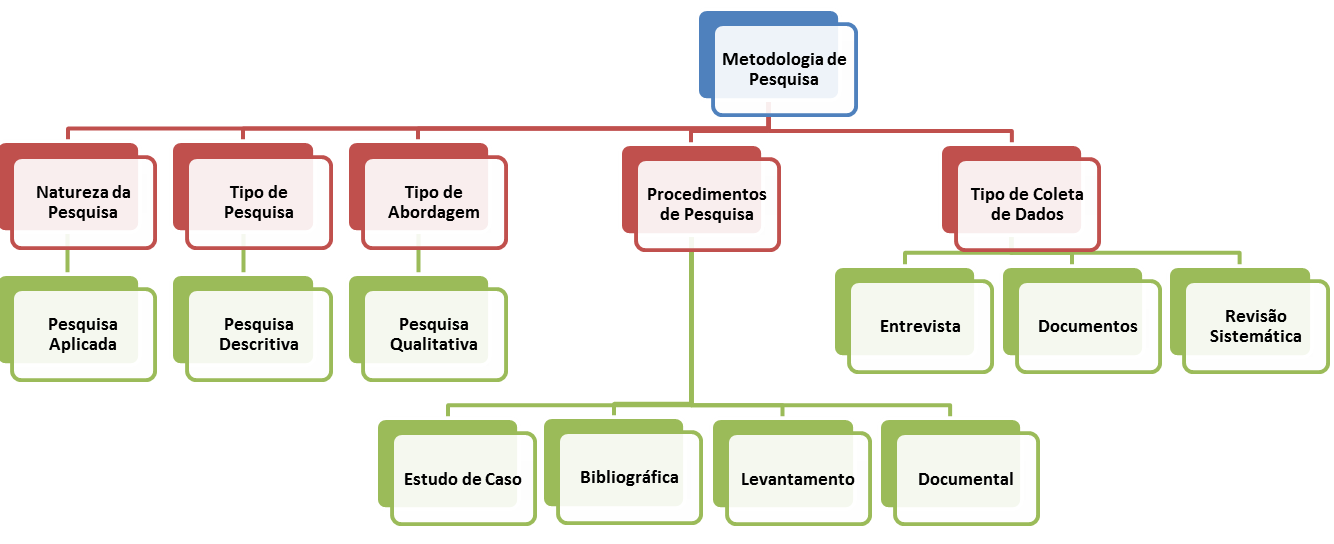
\includegraphics[scale=0.7]{figuras/metodologiapesquisa.png}
		\caption{Seleção de Metodologia de Pesquisa}
	\end{figure}

Nesta pesquisa, o esquema adotado compreende as fases: Planejamento; Coleta
de Dados; Análise e Interpretação dos dados, e Redação do Resultado. 

O Planejamento consiste na determinação da questão de pesquisa, a escolha da metodologia de pesquisa, a definicação das fases da pesquisa,  a definição dos procedimentos de pesquisa e das técnicas de coleta de dados, a construção do referencial teórico e a proposta do trabalho final.


Na Coleta de Dados são executados os procedimentos de pesquisa e as técnicas de coletas de dados a seguir:

\begin{itemize}
\item Pesquisa Bibliográfica: pesquisa realizada a partir de livros, dissertações e trabalhos relacionados à área de pesquisa.
\item Pesquisa Documental: pesquisa realizada a partir de documentos públicados por organizações públicas.
\item Estudo de Caso: utilizar um estudo de caso real de uma organização pública brasileira.
\item Entrevistas: dados serão coletados por meio de estrevistas semi-estruturadas para incremento do estudo de caso.
\item Documentos: técnicas de leitura dos documentos fornecidos pelo órgão público do estudo de caso será emprega para coleta de dados para análise.
\end{itemize}

A Análise dos Resultados diz respeito a fase em que os dados coletados são analisados e interpretados.

A Redação dos Resultados diz respeito a fase em que os resultados serão estruturados e concluídos.

\section[Organização do Trabalho]{Organização do Trabalho}

Este trabalho está organizado em cinco capítulos. Neste Capítulo 1 encontra-se a introdução do trabalho que consiste em: contexto do trabalho, a justificativa,  o problema, os objetivos e a metodologia de pesquisa adotada.

No Capítulo 2 - Contratações de Fornecedores de Desenvolvimento de Software - apresenta-se as principais informações referentes à Contratações de Fornecedores de Desenvolvimento de Software. Para isso, o capítulo é iniciado cum uma visão geral sobre a importância das contratação e suas principais características, posteriormente, é apresentado um resumo das legislações e processos relativos à Contratações de Serviços de Tecnologia da Informação.

No Capítulo 3 - Pensamento Lean - é apresentado os conceitos referentes ao Lean na Manufatura e ao Lean no Desenvolvimento de Software. Com este fim, é apresentado um breve histórico sobre o surgimento do Lean na manufatura e os seus principais princípios e práticas e, posteriormente, é apresentado como o Lean Manufatura foi adaptado para o desenvolvimento de software e para isso é abordado os princípios e práticas do Lean no Desenvolvimento de Software.